\documentclass[sigconf,anonymous,review]{acmart}
\usepackage[normalem]{ulem}


\usepackage{amssymb} % needed for: various symbols
\usepackage{amsmath} % needed for: math symbols
% http://tex.stackexchange.com/questions/229355/algorithm-algorithmic-algorithmicx-algorithm2e-algpseudocode-confused
\usepackage{algorithm} % this used as an environment for the algorithm code (linke figure and table)
\usepackage{algorithmicx} % this is used to write the pseudo code
\usepackage[noend]{algpseudocode} % this is for the layout of the pseudo code
\usepackage{tikz} % needed for: tikz pics
% \usepackage[inline]{enumitem}
\usepackage{xcolor}
\usepackage{xspace}
\usepackage{natbib}

\usepackage{graphicx}  
\usepackage{subfigure}
\newcommand{\TODO}[1]{{\bf \em \textcolor{red}{TODO: #1}\xspace}}
\newcommand{\sys}{NAME\xspace}

\begin{document}

\title{VIPOS: Virtualized Intermittently Powered Runtime Environment (``VIPRE''?)}
% \author{
% 	\IEEEauthorblockN{Amjad Yousef Majid, Przemys{\l}aw Pawe{\l}czak}
% 	\IEEEauthorblockA{TU Delft, Mekelweg\,4, 2628\,CD Delft, NL\\
% 	\{a.y.majid, p.pawelczak\}@tudelft.nl}
% }


\maketitle

\section{abstract}
\TODO{Need to re-write this to make it consistent with the story after we have the story in place}
Enabling battery-free devices is a mandatory step towards the environment friendly IoT. However, removing these large energy reservoirs (the batteries) makes the devices operate on an intermittent power supply, which make sustaining any long computation very challenging. correspondingly, there are two proposed approaches to enable long-running computations on intermittenly powered devices (IPDs): (i) Checkpointing based approach, where the volatile state of a program is frequently saved to the non-volatile memory and; (ii)  Task based approach, where a programmer splits the code into small idempotent modules. The Task based approach shows a better performance than the checkpointing approach. However, the task based method requires that the energy to execute any task must not exceed the maximum limit of the energy buffer. This limitation makes this solution a customized one that suits a particular energy buffer size. 

VIPOS enables code portability by means of virtualizing the task based model. If a code is written for a very small energy buffer, VIPOS is able to dynamically merge these tasks and constructs a bigger virtual task to improve the performance, reduce energy consumption and provides mean for code portability. 

\section{Introduction}
\label{sec:intro}
\TODO{VIPER: Virtualized Intermittent Programming model, Execution model, and Runtime environment}
\TODO{PREVIEW: Programming and Runtime Environment with Virtualized Intermittent Execution Windows}

Advances in processor efficiency along with the development of
energy-harvesting power systems has created a new category of devices that
require neither a battery nor a tethered power supply.  These devices operate
entirely using energy extracted from their environment, such as RF energy,
photovoltaics, and vibration.  Incorporating compute, storage, sensing, and
communication hardware, such energy-independent devices are a promising
candidate as the underlying technology for emerging internet of things (IoT)
applications, in- and on-body medical applications, and emerging applications,
like energy-harvesting nano-satellites.  

While promising, energy-harvesting devices present a unique design challenge in
that they operate only {\em intermittently} when energy is available.   An
energy-harvesting device buffers energy from its environment, e.g., in a
capacitor. When a threshold quantity of energy accumulates, the device begins
operating.  Harvestable energy sources typically produce relatively very little
power compared to a platform's operating power level.  A devices operates for a
brief period of time and when buffered energy is depeleted, shuts down and
begins recharging to later operate again.  Charge and discharge times vary by
device and some devices~\cite{wisp} may fail 10 to 100 times per second.

Software in an energy-harvesting system operates according to the {\em
intermittent execution model}~\cite{dino}, with bursts of execution that are
interrupted by failure periods. When power fails, a device loses its volatile
state (i.e., registers, stack, SRAM) and retains its non-volatile state (i.e.,
FRAM, Flash). While capturing periodic checkpoints~\cite{mementos,tictpl,quickrecall}
and sleep scheduling~\cite{dewdrop,hibernus,hibernusplusplus} help to preserve
execution progress, failures can leave volatile and non-volatile state inconsistent,
leading to unrecoverable failures~\cite{mspcdino,edb,edbtoppicks}.  

\TODO{Don't forget to include all the references in this section!}

%FRAM costs more than FRAM -- need to figure out how to execute out of SRAM
New programming and execution models~\cite{dino,ratchet,chain,alpaca} and
architecture mechanisms~\cite{clank, idetic, nvp} help avoid data
inconsistency.  New architectures require costly hardware changes and are
inapplicable to today's systems.  New programming models and compilers force
programmers to use new memory models~\cite{chain,ratchet}, which may inhibit
adoption.  New memory models may also increase the amount of non-volatile
memory accesses by requring non-volatile versioning~\cite{chain} or completely
precluding the use of volatile memory~\cite{ratchet}.  Increasing pressure on
non-volatile memory or precluding the use of volatile memory may degrade
efficiency; e.g., FRAM has a higher access energy and latency than
SRAM~\cite{alpaca,wisp}.  Commercially available devices are often provisioned
with much less SRAM than FRAM~\cite{wolverine,wisp} and effectively leveraging
the relatively high efficiency of SRAM is a key challenge for task-based
intermittent systems.

\TODO{concrete cost multiples here?}

%Task sizing is hard -- how to chop without risking inefficiency or non-term
Several recent programming efforts~\cite{alpaca,chain} proposed {\em
task-based} programming models, that require the programmer to statically
decompose their program into tasks.  A task is like a function with no callers
that can include arbitrary computation and, upon completion, is guaranteed to
have executed {\em atomically} and to have logically {\em committed} memory
updates.  The programmer expresses the flow of control from one task to another
and task control-flow may be input-dependent.  An important programming
challenge in task-based models is that the length of execution of a task is
limited by the total amount of energy that a device can buffer.  Assuming that
input power is negligible compared to operating power, a task will never be
able to complete if its execution consumes more energy than the system can
buffer.  Transitioning from one task to the next imposes a cost and excessively
small tasks may be inefficient.  Appropriately sizing tasks to ensure progress
and high performance is a key challenge for task-based intermittent systems. 

In this work, we develop \sys: a new programming and execution model that uses
{\em volatile memory virtualization} to leverage efficient volatile memory and
and {\em dynamic task coalescing} to efficiently execute tasks without
exceeding available energy.  \sys's memory virtualization mechanism uses a
device's SRAM as the working memory during a task's execution, populating the
SRAM with a page of data from FRAM as necessary at the start of the task.  At
the end of the task, the SRAM is committed back to FRAM using efficient DMA
block copies.  \TODO{Brandon sez: Is the next sentence what the system does?
Or are we doing paging?} When a task accesses data outside of a page in SRAM,
the task must fetch data from FRAM.  We explore two strategies. The first
strategy is {\em demand paging}, which swaps the SRAM page with a new page from
FRAM, buffering the swapped-out page until commit.  The second strategy is {\em
buffered direct access} \TODO{better name}, which directly reads and writes
FRAM relying on dynamic double-buffering to ensure memory is consistent at
commit.

\sys's dynamic task coalescing mechanism allows the programmer or a compiler to
intuitively decompose their program into small tasks that amortize fixed
per-task overheads, yet present no risk of exceeding device energy capacity. As
such a decomposition executes, \sys {\em coalesces} dynamically consecutive
tasks. Coalescing elides the commits of coalesced tasks by buffering multiple
tasks' updates in an FRAM commit buffer.  Periodically, as the span of the
coalesced task grows, \sys ends coalescing and commits the state of the
coalesced task.  If a power failure interrupts a sequence of coalesced tasks,
\sys adaptively reduces the number of tasks in that sequence that it will
coalesce, committing sooner in future executions.  Consequently, \sys's
coalescing mechanism allows a program to execute efficiently across a range of
energy buffer sizes, avoiding transition overheads in larger buffers, and
ensuring progress in smaller buffers. \TODO{articulate this last point better}

We evaluated our system on a collection of benchmark programs taken from the
literature, and compare directly to prior work, showing that \sys has high
performance and can flexible target a variety of platforms without recompiling
the code.  We further demonstrate the efficiency and versatility of \sys with
an end-to-end evaluation of a sensing and data processing application deployed
in a lab environment \TODO{blah blah blah eval}.

\TODO{Bullet contribs if there's space}





\section{Old Introduction}
	Intermittently powered devices (IPDs) are battery-less devices that utilize the ambient energy to sense, compute and, communicate. For example, Wireless Identification and Sensing platform WISP \cite{wisp} uses the RF signal power to drive its computation and communication. Because of the reliance of TPDs on intermittent power supply, the harvested energy when it is available, their programs are susceptible to a very frequent power interrupts, in the order of tens of millisconds~\cite{}. Therefore, these devices require a different software execution model that complies with the nature of a discontinuous power supply. 

	The intermittent (discontinuous) execution model defines a program execution as cumulative discrete process. The main difference between the intermittent and the conventional (or continuous) execution models is that, a power failure is seen by the continuous model as an \emph{exception} that may reset the progress of a program to its beginning. Whereas, in intermittent execution a power failure is regarded as a temporary \emph{pause} to the execution that may result in some progress degradation. Generally we can classify the intermittent execution model into: 
	\begin{itemize}
		\item \emph{Sequential Execution Model}:
			Under this model a program is seen as one big idempotent operational region that has one common context. Generally, The progress of the program is saved and updated by means of checkpointing---where all the program context (e.g. CPU registers, the stack and the global variables) is saved to a non-volatile memory. Normally, the sequential model relies on a hardware assistant to measure the voltage level in the energy reservoir to place a checkpoint~\cite{mementos, harvOS, hibernus}. The benefit of this model is that it does not require code modification by a programmer. However, it has a number of drawbacks: (i) It suffers from significant overhead \cite{chain}; (ii) the programmer should not access the non-volatile memory to guarantee the consistency of the memory~\cite{xxxx}; and (iii) it restricts the IPDs to run only a single application~\cite{inos}. 
		\item \emph{Modular Intermittent Execution Model}:
			At the heart of this model is the concept of an idempotent task. The idempotent task is C function that does not have arguments and does not return a value. This task uses a well defined interface to interact with the non-volatile memory. Therefore, it tolerates arbitrary number of power interrupts. This model, generally, produces less overhead~\cite{chain} and allows multiple applications to run on an IPD by interleaving their tasks~\cite{inos}. However, it obviously requires code modification---for example, if an algorithm is written according to the continuous execution model it has to be splitted, by a programmer, into small tasks to run under the modular intermittent execution model.
	\end{itemize}

Despite that the superiority of the Modular Intermittent Execution model, it is still a static approach that completely depends on a programmer's estimation which is mostly result in a sub-optimal code devision. Moreover, this model can only consider a single hardware configuration and it does not take environment changing into considerations. 




% Energy source


% The intermittent execution is cumulative discrete process. The intermittent execution model is only able to execute a few number of instructions, as compared to the conventional (continuous) model, before its progress is terminated. Therefore, the intermittent execution model adapts an execution progress state saving mechanism. This mechanism is realized either by means of a checkpoint~\cite{}, where all the context of the program is saved into non-volatile memory. Or 

% This progress state saving mechanism is normally injected into a program either by a compiler~\cite{}. A compiler injects trigger pointers to checkpoint (save) the context of the program into the non-volatile memory.  or it is added by a programmer~\cite{chain}. [compare these two approaches]...

% We define virtualization within the context of intermittent execution as utilizing the volatile memory instead of non-volatile when the intermittent execution model attempts to access the non-volatile memory. 


\subsection{Problem Statement}
How to approach the optimal task size given an unknown energy buffer size and environment conditions? 
	 \begin{enumerate}
		 \item How to eliminate the need for the hardware support while enabling the Modular Intermittent Execution model to dynamically adapt its task size?
		 \item How to enable code portability under the Modular Intermittent execution model? 
		 \item How to reduce the energy consumption of executing a task? 
	\end{enumerate}

\subsection{Why not Adapting Current Approaches}
Here we highlight the challenges of adapting the state-of-the-art proposed methods to enable the execution of dynamic task sizes. 
%
%	\begin{figure}[t]
%	    \centering
%	         \subfigure[Chain: Sequential task execution flow control.]{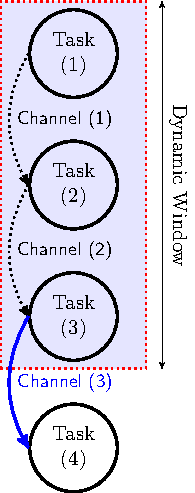
\includegraphics[width=0.35\columnwidth]{figures/dynamic-chain.pdf} \label{fig:DynamicChainSeq} } 
%	         \subfigure[Chain: Random task execution flow control.]{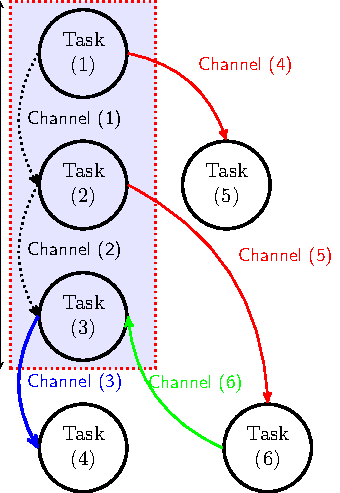
\includegraphics[width=0.61\columnwidth]{figures/dynamic-chain-2.pdf} \label{fig:DynamicChainRan}}
%	    \caption{Task flow control of Chain}
%	    \label{fig:DynamicChain}
%	\end{figure}


\noindent\textbf{Chain: Tasks and Channels for Reliable Intermittent Programs } \\
Some of the main problems in modifying Chain to support dynamic task's size are:

\begin{itemize}
	\item \emph{Multi-versioning system:} Chain defines for each task its own input that is not shared with other tasks. This design decision makes the benefit of merging tasks of less importance since each task is interacting with its own variables. 
	\item \emph{Direct FRAM system:} Chain tasks directly access FRAM which is more energy expensive Than SRAM. As result of being multi-versioning system that directly interacts with FRAM, Chain has a significant energy consumption overhead. 
	\item \emph{Irreversible tasks transitions:} According to the Chain programming model, each task calls the next one. The transition is done through functions calls and manually clearing the stack, to prevent the stack overflow problem. This approach make all the transitions firm ones which prevent task merging.
	\item \emph{All channels are required:} Fig.~\ref{fig:DynamicChainSeq} shows that if the task control flow is a circular with no branches then task merging is possible. Moreover, all the intra-merged-tasks channel can be committed to SRAM instead of FRAM to save energy. However, this execution path is only a special. If the general case (see Fig.~\ref{fig:DynamicChainRan}) is considered then leaving out the intra-merged-task channels might result in data inconsistency---If an application tries to access a merged task from the middle after a power interrupt then the input for that task is not ready which result in an incorrect execution. 


\end{itemize}


\noindent\textbf{Alpaca: Intermittent Execution without Checkpoints} \\
Some of the main problems in modifying Alpaca to support dynamic task's size are:

\begin{itemize}
	\item \emph{Privatization:} The core concept of Alpaca is privatization. Privatization depends completely on detecting the variables that have a Write-after-read dependency within the scope of a task. Therefore, if tasks are on-demand merged the scope of these dependencies are changed and the static analysis to privatize these variables is not valid anymore and data consistency can not be preserved.  

	\item \emph{Irreversible tasks transitions:} Similar to Chain problem. 

\end{itemize}

\noindent\textbf{Virtualizing Modular Intermittent Execution Model}

		An Intermittently executed program, as seen by the modular intermittent execution model, is a chain of tasks with a firm transition from one to another. 
		Virtualizing this model means softening a number of transitions, by keeping the state of the execution progress in the volatile memory, to construct a bigger \emph{virtual task} to reduce energy consumption. Ideally, the size of the virtual task should match the length of a continuous interval of the intermittent power supply for the best performance. Another form of virtualization can be achieved by reducing the number of non-volatile memory accesses. This can be done by having a temporary copy of a global variable in the volatile memory (similar to the catching principle) and a task interacts with it and updates it before writing back the most recent value to the non-volatile memory during the commit process.

		In this paper we are introducing VIPOS a runtime library the implement the Virtualed Intermittent Execution Model. VIPOS adapts two methods for data protection. One relies on a virtual buffer and the other uses the Direct Memory Access (DMA). VIPOS is able to approach the optimal tasks devision during the runtime. VIPOS reduces an application execution time by XX and the energy by XX. 


\subsection{Contributions}
	 \begin{enumerate}
		 \item We have developed an algorithm that is able to determine the size of a virtual task based on the history of the execution of an application. 
		 \item We enable efficient code portability by requiring that a real task to small and merging them during the execution.   
	\end{enumerate}


 \section{Preliminary Results}
 \label{sec:prelResults}

\begin{figure}[t]
    \centering
         \subfigure[The energy cost of FRAM/SRAM writes operations.]{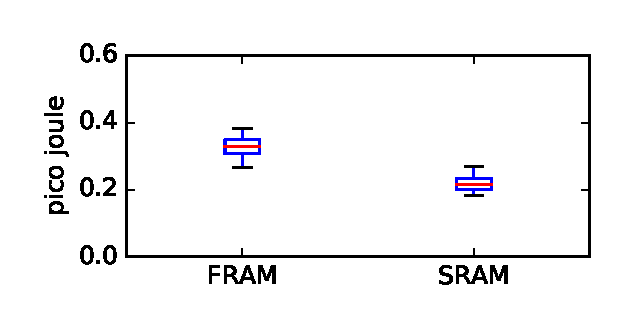
\includegraphics[width=0.48\columnwidth]{figures/fram_write.eps} }
         \subfigure[The energy cost of FRAM/SRAM read operations.]{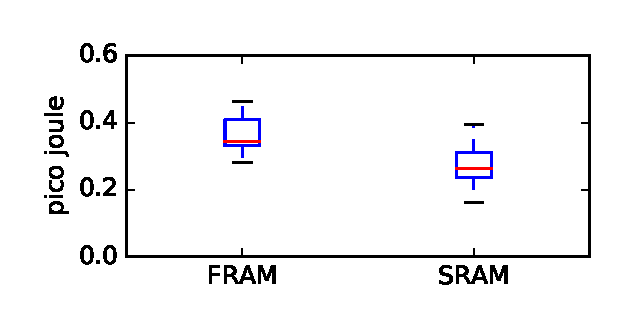
\includegraphics[width=0.48\columnwidth]{figures/fram_read.eps}}
    \caption{The energy cost of accessing volatile/non-volatile memory}
    \label{fig:framEnergy}
\end{figure}

Since the Intermittent execution models rely on the non-volatile memory to enable long-running operation, it is important to characterize the energy consumption of accessing this type of memory as compare to the volatile one.

Four applications are developed to measure the energy consumption of \emph{Accessing} the FRAM and SRAM of the MSP430FR5969 microcontroller~\cite{xxx}. The interference free debugger (EDB)~\cite{xxx} is used as the energy measurement tool. The EDB probes the energy buffer before and after accessing the FRAM/SRAM 1600 times, This large number of FRAM access is used to increase the reliability of the results generated by the used measurement tool (e.g. reducing the effect of the quantization error).  The energy buffer is charged, using the EDB, to $\approx$ 2.45 volts \textbf{only} at the beginning of the execution and of the programs. The write operations were performed by writing literal values, random numbers, to the memory. However, a read operation must be followed by a write operation, therefore, we chose to write a read value to SRAM. Fig.~\ref{fig:framEnergy} shows that an FRAM access equals $\frac{3}{2}$ SRAM access~\footnote{We would like to mentioned that TI has already mentioned in this document~\cite{xxxx} that FRAM write access is more energy expensive than SRAM write access. However, TI does not quantify the energy overhead.}. Therefore, reducing FRAM access is desirable when developing  energy limited software solution  




\section{VIPOS: Virtualized Intermittently Powered Runtime Environment}
VIPOS is runtime library that facilitates tasks navigation and preserves data/memory consistency of the IPDs. It is able, on-demand, to merge tasks to reduce the number of commits to the non-volatile memory.

\subsection{VIPOS: Data/Memory Protection Methods}
VIPOS data consistency preservation methods are designed with goal of minimal interaction between the CPU and FRAM to reduce energy consumption (see Section~\ref{sec:prelResults}). These data/memory protection methods enables VIPOS to tolerate arbirary number of power failures. 

	\subsubsection{Virtualized Operational Buffer}

		\begin{algorithm}[t]
			\caption{Virtualized Operational Buffer}
			\label{algo:virtuBufWrite}
			\scriptsize
			%\small
			\begin{algorithmic}[1]
				\State $var \in \text{\{global variables\}} $ 
				\State \label{lst:virtuBufWrite:line:begin}\Call{Virtual Task()}{} 
				\While { \textit{executing} } \Comment{Execution stage}
					\State $var$  $\rightarrow$ \textsf{volatile buffer} \label{lst:virtuBufWrite:line:output}
					\If { $var$  in \textsf{ volatile buffer} }				\label{lst:virtuBufWrite:line:inputBegin}
							\State $var$  $\leftarrow$  \textsf{volatile buffer} 
						\Else 
							\State $var$  $\leftarrow$  \textsf{FRAM}		\label{lst:virtuBufWrite:line:inputEnd}
						\EndIf

					\If {power interrupts}
						\State back to \ref{lst:virtuBufWrite:line:begin}
					\EndIf
				\EndWhile

				\While{  $\textsf{volatile buffer}\not=\emptyset$  } \label{lst:virtuBufWrite:line:commitBegin} \Comment{ First phase commit}
					\State \textsf{volatile buffer} $\rightarrow$  \textsf{persistent buffer}
					\If {power interrupts}
						\State discard \textsf{persistent buffer}
						\State back to  \ref{lst:virtuBufWrite:line:begin} 
						\State   \label{lst:virtuBufWrite:line:commitEnd}
					\EndIf
				\EndWhile 

				\While{ $\textsf{persistent buffer}\not=\emptyset$ } \label{lst:virtuBufWrite:line:SecCommitBegin} \Comment{Second phase commit}
					\State \textsf{persistent buffer} $\rightarrow$ FRAM 
					\If {power interrupts}
						\State Continue
					\EndIf
				\EndWhile 
				\State     \label{lst:virtuBufWrite:line:SecCommitEnd}
				\State return
			\end{algorithmic}
		\end{algorithm}


		Since accessing FRAM is more energy expencive and slower than accessing SRAM, preventing frequent access to FRAM (i.e. during looping operations) is desireable. Therefore, the first proposed protection method utilizes a volatile buffer that holds temporary all the outputs of a virtual task (see Algorithm~\ref{algo:virtuBufWrite} line~\ref{lst:virtuBufWrite:line:output}). Consequently, a virtual task must first attempt to read a global variable from the volatile buffer before trying to obtain the value from the non-volatile memory (see Algorithm~\ref{algo:virtuBufWrite} lines~\ref{lst:virtuBufWrite:line:inputBegin}-\ref{lst:virtuBufWrite:line:inputEnd}) to ensure a correct execution progress and the consistency of the memory. Once the execution of a virtual task is done, the first phase of the commit process is started by copying the volatile buffer to a persistent buffer (see Algorithm~\ref{algo:virtuBufWrite} lines~\ref{lst:virtuBufWrite:line:commitBegin}-\ref{lst:virtuBufWrite:line:commitEnd}). If the power is interrupted the persistent buffer must be discarded and the execution must start again from the beginning of the virtual task. In another words, the first phase commit must be performed atomically to preserve the consistency of the output of a virtual task. The second phase commit is a power failure immune precess that is responsible for distributing the global variables to their final locations and make the non-volatile memory consistent and synchronized with the computation progress (see Algorithm~\ref{algo:virtuBufWrite}lines~\ref{lst:virtuBufWrite:line:SecCommitBegin}-\ref{lst:virtuBufWrite:line:SecCommitEnd}).


	\paragraph{Virtualized Operational Buffer: Implementation} 

		We implement a reference implementation of VIPOS that uses virtualized Operational buffer to protect the data against power failure. 
		\paragraph{Virtual Buffer}
			We realized the virtaulzed buffer as a volatile hashed table of linked lists. The hashing technique was chosen to reduce the buffer searching time and the linked lists are used to prevent data loss when there is a conflict between multiple variables---If two variables have the same hash value they will occupy the same cell, however, with linked list a new node will be created for each variable to resolve the conflict and protect the data. The hashing function is based on the observation that the virtual addresses of the memory cells have approximately a flat distribution over the memory addressing space and the fact that each entry, of the virtual table, has the address and the value of a variable. As such, by using the least significant bits as an index to access the virtual buffer the hash function distributes its inputs uniformly in the virtual buffer. Accordingly, the linked lists search time, on average, is reduced.

		\paragraph{Persistent Buffer}
			The persistent buffer is implemented as static array of tuples, where each tuple holds  the address and the value of a variable. This data structure is very suitable for the second phase commit where each element has to be committed to its finial location. However, the complexity of committing this buffer is of size $O(N)$, where $N$ equals the length of the buffer. Therefore, the size of the buffer can have dramatic effect on the performance of VIPOS---On one hand, if the size of the buffer is small the buffer overflow problem will be very serious. On the other hand, if the size of the buffer is large VIPOS will experience a significant performance degradation. However, by observing the type of the information that this buffer holds, namely memory addresses, we can, on average, reduce the complexity of committing this buffer by defining the \emph{effective size} of the buffer to be the size of the buffer up to the first cell that holds an invalid memory address. Moreover, since this buffer is in FRAM which is much bigger than SRAM its size can be relatively big. 

		\paragraph{Virtualized Operational Buffer: delay analysis}[initial results]

		\begin{figure}[t]
			\centering
			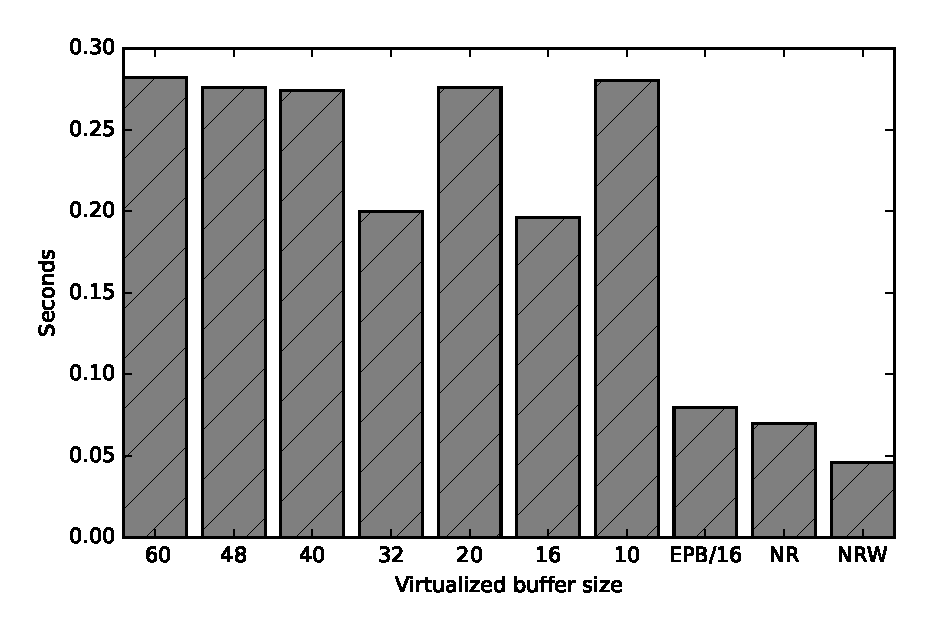
\includegraphics[width=\columnwidth]{figures/virtual_buffer_size.eps}
			\caption{VIPOS based on virtualized Operational Buffer. It runs the decompression application with different buffer configurarions. EPB: Enhanced Persistent Buffer. NR: no read operation from the buffer. NRW: not read or write operations from the buffer.}
			\label{fig:virtOperationalBuf}
		\end{figure}

			To analyze the performance of VIPOS versus the sizes of the virtual buffer and the persistent buffer we setup the following experiment. We let IPOS to run the decompression application---until the data decompression is completely finished---and we capture the execution time using a logic analyzer~\cite{xxx}. The results presented in Fig.~\ref{fig:virtOperationalBuf} show the VIPOS has its best performance when the virtual buffer size is 16, where the execution time was $\approx$196 ms. 

			All the experiments were done with a persistent buffer of size 100. However, the bar labeled with "EPB/16" in  Fig.~\ref{fig:virtOperationalBuf} shows the effect of the enhanced commit process that uses the buffer effective size instead of the buffer maximum size. We see that the execution time is reduced to $\approx$80 ms. Furthermore, we quantized the overhead of the read operations from the buffer, by eliminating this operation, and the bar labeled with "NR" shows that it cost  $\approx$10 ms. Moreover, the overhead of the read and write operations is $\approx$34 ms as compared to VIPOS best performance, see the bar labeled with "NRW" in Fig.~\ref{fig:virtOperationalBuf}. 


\subsubsection{ Direct Memory Access Based Protection Method (better name is needed)}
%
	\begin{figure}[t]
		\centering
         \subfigure[The time needed to transfer a block of data using pointers versus Direct Memory Access (DMA).]{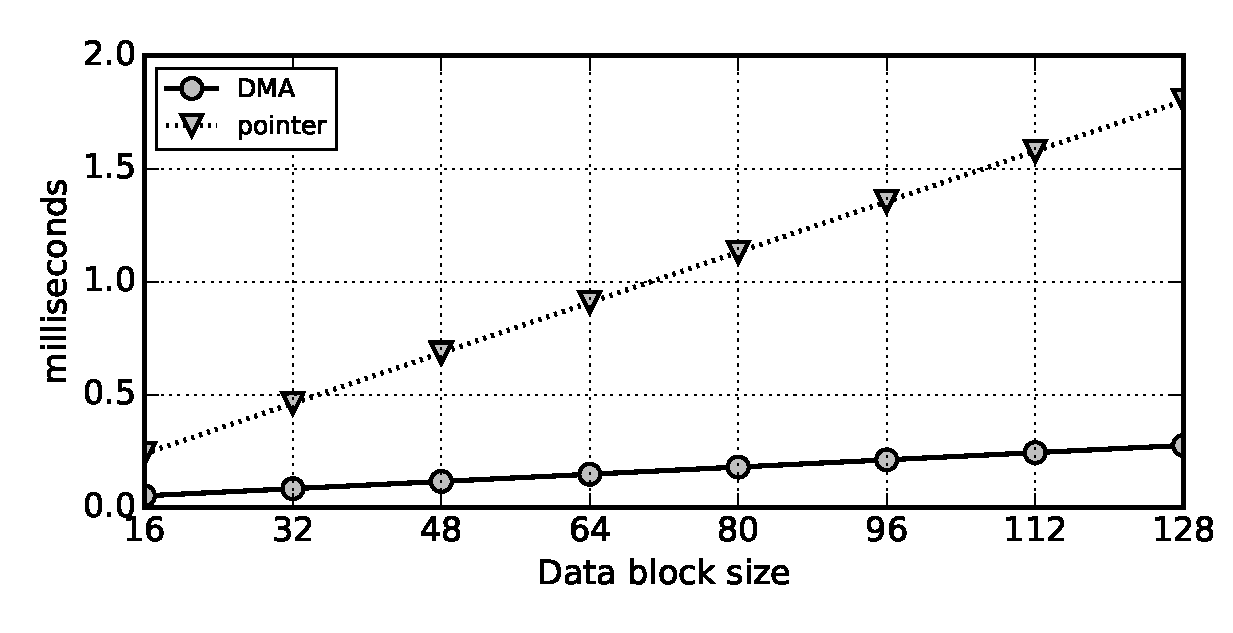
\includegraphics[width=0.48\columnwidth]{figures/dmaSize.eps} }
	     \subfigure[The energy needed to transfer a block of data using pointers versus Direct Memory Access (DMA).]{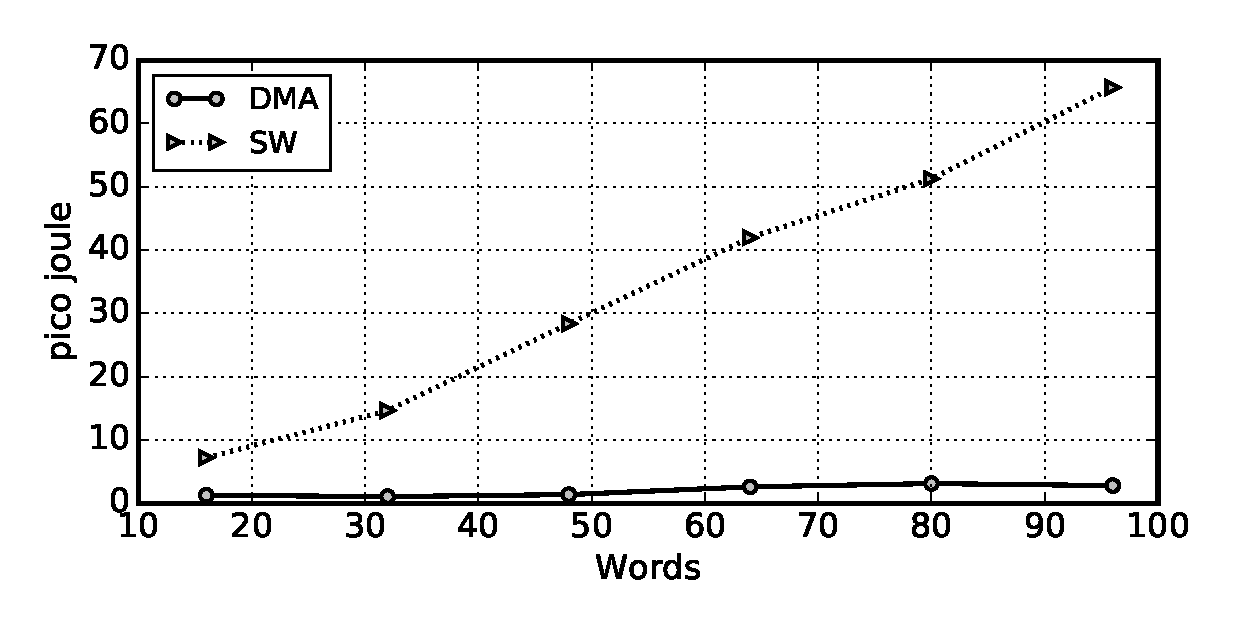
\includegraphics[width=0.48\columnwidth]{figures/energyConsumptionDMA_SW.eps}}
		\caption{Time and energy consumption of moving a block of data from SRAM to FRAM}
		\label{fig:dmaTimeEnergy}
	\end{figure}
%
	Since accessing/updating buffers is more costly than directly accessing FRAM, at least without specialized hardware~\cite{clank}, we introduce the second method to apply the virtualization principle to the Modular Execution Model. This method utilizing the Direct Memory Access (DMA) Module. As Fig.~\ref{fig:dmaTimeEnergy} shows that DMA is much more efficient in transferring a block of data than the conventional (pointer based) way from the energy and time perspectives. 

	This method combines a number of techniques to preserve the persistence and consistency of the data. It backs up the status of the global variables in the non-volatile memory, and double buffers them to guarantee their consistency. Furthermore, on each power up it populates the global variables in the volatile memory from the most recent back up in the non-volatile memory to enable a faster task execution since the task does not need to interact with non-volatile memory which is generally slower and more energy expensive.   



\subsection{VIPOS: The Virtualizing Engine}
\subsubsection{Power Interrupt Immune Scheduler}
It utilizes a persistent circular buffer (persistent linked-list) to keep the state of a program across power failures. VIPOS provides an API to enable a programmer to have a full control over the execution flow of the program, i.e. (un)blocking a task or re-execute the same task which is particularly important in the intermittent execution to emulate a persistent loop. 

\subsubsection{Task Merging Algorithms}

\paragraph{Fixed Virtual Task Size} [better name needed]

	\begin{algorithm}[t]
		\caption{Fixed virtual Task size}
		\label{algo:fixVirtTask}
		\scriptsize
		%\small
		\begin{algorithmic}[1]
			\State $VT \subset \text{\{VIPOS Tasks\}} $  \Comment{$VT:$ Virtual Task}
			\State VTS : VT size
			\State MVTS: maximum VT size
			\vspace{0.1cm}

			\While {$True$}
				\State $VT \leftarrow VT_{next}$
				\vspace{0.1cm}
				\While {execute $VT$} 
					\If { $\text{power failed twice}$ }				
							\State $VTS--$  
							\State $ MVTS = VTS $
						\EndIf
				\EndWhile

				\vspace{0.1cm}
				\If {$ \text{All tasks executed}$}
					\If{$VTS < MVTS$}
					\State $VTS++$
					\EndIf
				\EndIf
			\EndWhile
		\end{algorithmic}
	\end{algorithm}



\begin{figure}[t]
	\centering
	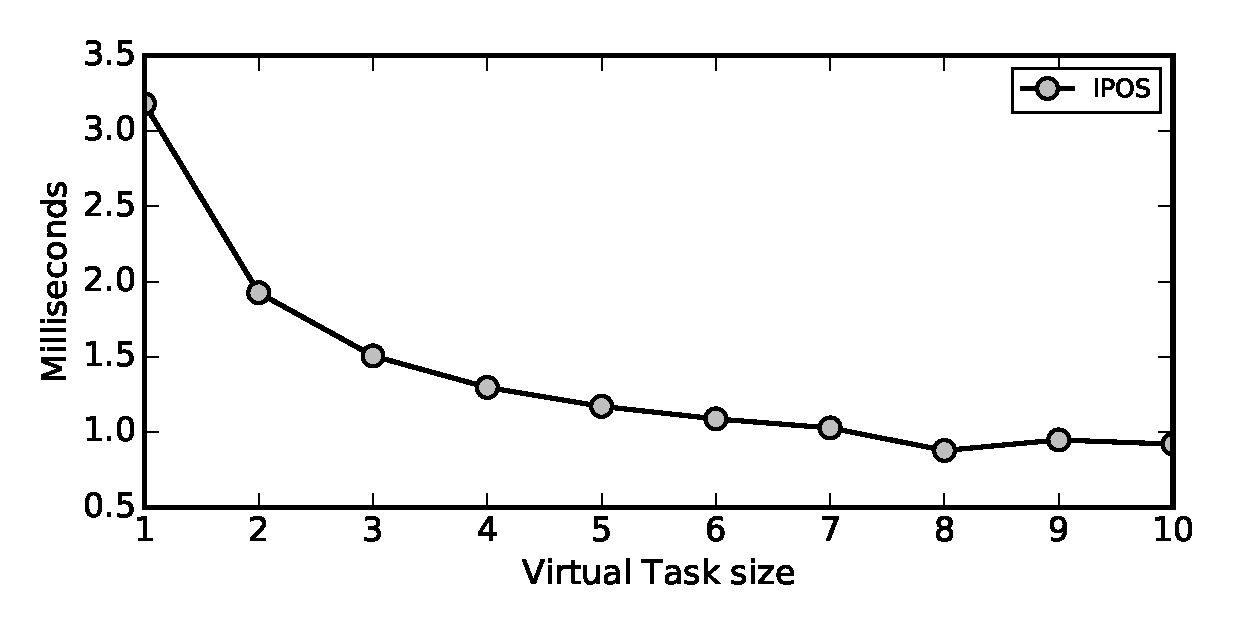
\includegraphics[width=0.7\columnwidth]{figures/virtualTaskSize.eps}
	\caption{Size of the virtual task versus the execution time of a dummy application that contains 12 empty tasks.}
	\label{fig:virtualTaskSize}
\end{figure}

VIPOS is able to virtually merge tasks to construct a bigger virtual task and commit the state of the virtual task instead of the individual real tasks. 
Fig.~\ref{fig:virtualTaskSize} show the benefit of virtualizing the Modular Intermittent Execution Mode (MIEM) in the best case scenario (continuous power supply). 

Remark: A less obvious benefit of visualization is that it can enable a secure computation. By increasing the size of the virtual task, the energy in the super-capacitor will not be enough to finish the execution of the virtual task. Therefore, without the interrogator being close to the intermittently powered device and charging rate is not negligible as compared to the discharging rate this computation will not be finished. As such, virtualization can add a layer of security to the computation.

\section{Results}
We compare the performance of VIPOS against a state-of-the-art intermittent execution approach. For this purpose, we used two different applications: (i) A data decompression application, which utilizes Huffman decoding technique to decompress 100 byte of data.; (ii) A discrete Fourier transform (DFT) application that uses two different resolution (4 and 8 bites) to analyze a randomly generated signal. 

\subsection{Continuous Power Supply}

\begin{figure}[t]
	\centering
	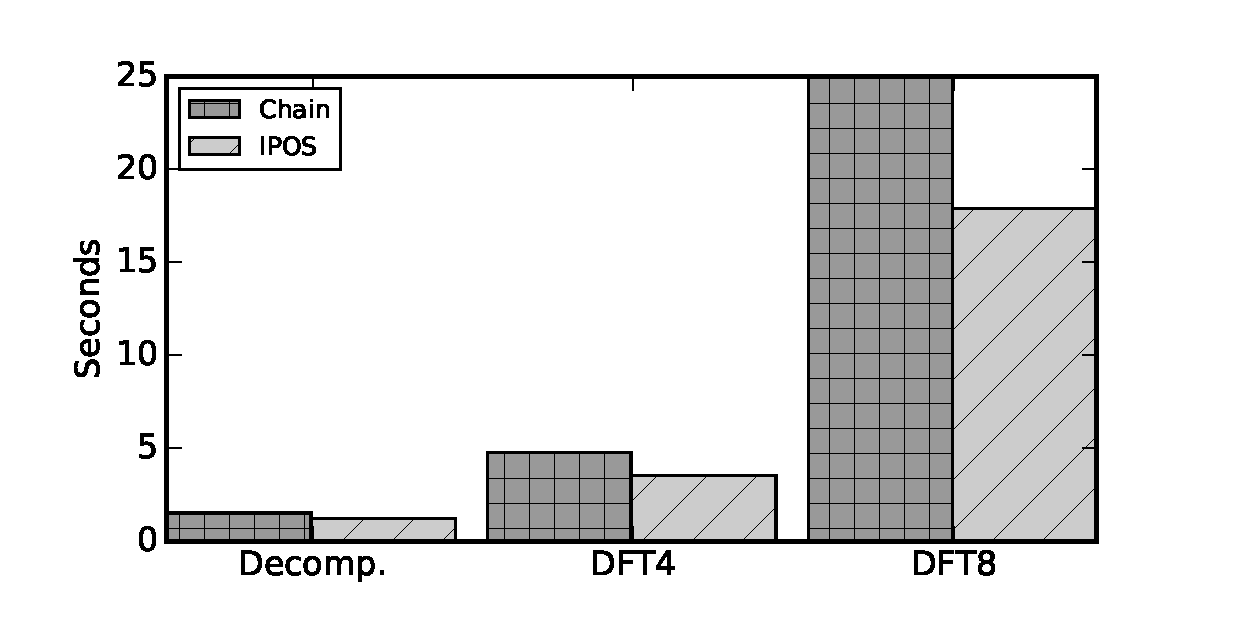
\includegraphics[width=0.7\columnwidth]{figures/executionTime.eps}
	\caption{Time to complation of VIPOS versus Chain. Decomp: Data decompression application. DFTx: Discrete Fourier Transform.}
	\label{fig:IPOSPerformance}
\end{figure}

Fig.~\ref{fig:IPOSPerformance} shows that VIPOS requires a shorter execution time to execute an application under the MIEM. The size of the virtual task that VIPOS uses equals One real task, in other words, no visualization is applied.

\subsection{VIPOS Operational Buffer Versus VIPOS DMA}[place holder]
			\begin{figure}[t]
				\centering
				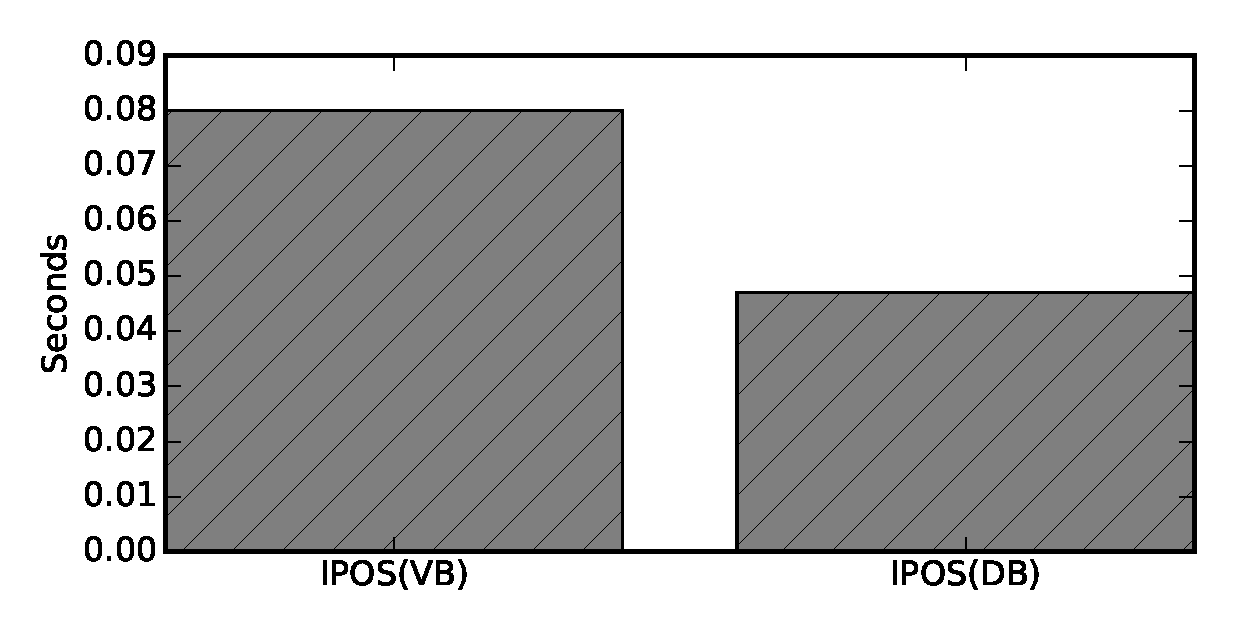
\includegraphics[width=0.7\columnwidth]{figures/ipos_virtualizedBuffer_overhead.eps}
				\caption{Virtualized Oprational buffer overhead.}
				\label{fig:virtualBuffer}
			\end{figure}


\subsection{Intermittent Power Supply}
...

\bibliographystyle{abbrvnat}
\bibliography{bib}

\end{document}
